% #############################################################################
% This is Chapter 3
% !TEX root = main.tex
% #############################################################################
% Change the Name of the Chapter i the following line
\fancychapter{State-Of-The-Art}
\clearpage
% The following line allows to ref this chapter
\label{chap:chap003}

In this chapter (Chapter~\ref{chap:chap003}), the document provide an overview on relevant literature works to the content of this thesis.
The document outlines the role of intelligent agents and how other authors are handling their work in various steps of the clinical workflow, including novel interactive systems in medical imaging, application of \ac{HCI} techniques in the domain and \acp{UI} with \ac{AI} methods behind.
To substantiate this thesis, the next sections will summarize important contributions in the particular domain of medical imaging and the role that \ac{HCI} and \ac{AI} topics are playing in this context.

\section{Literature Challenges}
\label{sec:sec003001}

Medical imaging systems allow the end-user to diagnose several modalities, such as \ac{MG}, \ac{US} or \ac{MRI}, from a seamless retrieval medical imaging data~\cite{faraji2019radiologic, seifabadi2019correlation}.
By bringing those modalities together, it offers new possibilities for quantitative imaging ({\it e.g.}, {\it radiomics}) and diagnosis but also requires specialized data handling, post-processing and novel visualization methods~\cite{Igarashi:2016:IVS:2984511.2984537, Ocegueda-Hernandez:2016:CMN:2876456.2879485, Sousa:2017:VVR:3025453.3025566}.
In the clinical domain, medical imaging tools can help experts make better decisions~\cite{Lopes:2017:UHC:3143820.3144118}, {\it e.g.}, by identifying cancer prognostics among the available multi-modal data~\cite{lopes2018interaction}.

A wide range of new contributions for medical imaging systems exist, providing clinicians with the knowledge to enhance the clinical workflow~\cite{Cai:2019:HTC:3290605.3300234, edge2019clinical}.
From systems that supply potential information~\cite{10.1145/3399715.3399744, 10.1145/3206505.3206555}, to decision-making systems~\cite{10.1145/3290605.3300468, 10.1145/3359206}, these new contributions are improving the diagnostic decisions of medical professionals~\cite{hwang2019artificial}.
Although several studies have shown that \ac{AI} systems can reduce medical error and improve outcomes~\cite{Cai:2019:HTC:3290605.3300234, Cai:2019:EEE:3301275.3302289}, one traditional difficulty is the lack of user trust and acceptance~\cite{https://doi.org/10.1002/mp.13562}.
On the one hand, experts may resist using a system if it does not capture the nuances of their mental models or provides relevant context~\cite{khairat2018reasons, kohli2018cad, yang2016investigating}.
On the other hand, clinicians are known to resist changes and new tools~\cite{10.1145/3132272.3134111, gagnon2014electronic}, an issue that has an impact in their workflow.

Despite the breakthroughs and progress in the context of \ac{AI} in medical imaging, one challenge regarding \ac{DL} approaches is its `black box' characteristics~\cite{10.1007/978-3-030-50334-5_4, 10.1145/3306618.3314293}.
Due to the high degree of complexity of \ac{DL}-based approaches such as \acp{NN}, there is no inherently comprehension understanding of the internal processes~\cite{8851763}.
\ac{AI} systems that suffer from this problem are often referred to as opaque~\cite{zednik2019solving}.
Hence, there is the trade-off between performance and explainability: while performance of models increase, the explainability of these approaches decrease~\cite{gunning2017explainable}.
In order to achieve higher transparency, new techniques to improve the interaction of humans and \ac{AI} must be addressed.

In this section, the document focus on understanding different aspects and challenges that other authors surpassed for the integration of their systems into the medical workflow.
In particular, their work demonstrates how an interactive system can directly address the above mentioned issues during medical imaging diagnosis.
The next section, introduce the topic of \ac{HAII}, as well as several related works, explaining the importance of the topic to this thesis work.

\section{Human-AI Interaction}
\label{sec:sec003002}

Applications of \ac{HAII} collaboration~\cite{dellermann2019future} in complex domains are subject to the following two issues:
(1) trust, transparency and accountability of the involved \ac{AI} agent~\cite{10.1145/3290605.3300233}; and
(2) user's ability to understand and predict agent behavior, {\it i.e.}, explainability and intelligibility~\cite{Cai:2019:EEE:3301275.3302289, gunning2017explainable, miller2018explanation}.
Forming accurate mental models of the \ac{AI}-assisted is useful for:
(i) representing the clinician's belief about what the system can do, acquired via interviews and observations, instruction, or inference;
(ii) mapping between the observable features of the developed framework and the functionality perceived by the user; and
(iii) the prediction for anticipating the \ac{AI} output in a given scenario.

In that context, several studies in user expectations~\cite{Kocielnik:2019:YAI:3290605.3300641, leung2019health} are postulating that user satisfaction and acceptance of a system is directly related to the difference between initial expectations and their actual experience.
Specifically, expecting more than the system can deliver will decrease user satisfaction and lead to the rejection of the system.
Hence, in the proposed work of this thesis a technique was created, based on the following contributions:
(a) providing users a new control feature on the introduction of \ac{AI} methods among medical imaging diagnosis~\cite{pesapane2018artificial}; and
(b) the impact of the clinicians' {\it behaviour}, as well as the impact in professional practice~\cite{Challen231}.
In the end, the final goal was to achieve more accurate expectations of each intelligent agent capabilities, addressing these potential gaps.

The growing prevalence of \ac{DL} models and their use in decision-making have led to increasing demands for more transparent and explainable results~\cite{10.5555/3305381.3305576}.
However, the interpretation of \ac{DL} models is challenging due to their complexity and often opaque internal state.
Thus, the \ac{ML} community has produced a myriad of algorithmic methods to explain their inner working~\cite{Shakerin_Gupta_2019, 10.1145/3329859.3329878}.
These methods aim to explain the model prediction outcome with two main reasons:
(1) for a single input data point~\cite{10.1145/2939672.2939778}; and
(2) for a set of data points in a predicted class~\cite{pmlr-v80-kim18d}, often by perturbing the inputs of the model and watching how the model response to changes.
Across this work, there is a clear need to ensure usability and efficacy with real users~\cite{10.1145/3173574.3174156}.
Consequently, a recent hype in \ac{HCI} research has studied what the end-user actually desire to understand the \ac{ML} results, as well as how that transparency affects user attitudes and behaviour.
Hence, the final outcomes are also (hopefully) improved which answers to what questions the user may desire to ask the \ac{AI} system.

Recent works on accountability and fairness have proposed the use of short records with trained \ac{ML} models revealing their intended use, details of their performance evaluation of procedures, and the potential biases that they may embody~\cite{10.1145/3351095.3375709, 10.1145/3287560.3287596}.
Additionally, others have studied whether people's trust varies depending on the stated accuracy of the model and how it differs from observed accuracy in practice~\cite{10.1145/3290605.3300509}.
In this thesis, the document builds on a growing interest in studying the broader, global aspects of model transparency, and conducts a deep exploration of these issues within the domain of decision-making in medical imaging.
The following section will discuss recent advances on the introduction of \acp{CDSSe} in the medical workflow.

\section{Clinical Decision Support}
\label{sec:sec003003}

Most of the best performing \acp{CDSSe}\footnotemark[8] rely on \ac{ML} algorithms that learn specific tasks from training data.
The field recently gained enormous interest, mostly due to the practical successes of \ac{DL}~\cite{meacham2019towards}.
The rapid and widespread development of \ac{DL} methods supports a wide range of image analysis tasks, including classification, detection, and segmentation \cite{lecun2015deep}.

%%%%%%%%%%%%%%%%%%%%%%%%%%%%%%%%%%%%%%%%%%%%%%%%%%%
\footnotetext[8]{The term was designated for computer applications that are designed to aid clinicians in making diagnostic and therapeutic decisions for patient care. In this thesis, we use this definition to define it as active knowledge systems for clinical advice.}
%%%%%%%%%%%%%%%%%%%%%%%%%%%%%%%%%%%%%%%%%%%%%%%%%%%

\ac{DL} methods rely on large annotated datasets to learn essential and to discriminate image features for each specific task, with performances matching and even surpassing humans~\cite{esteva2017dermatologist, McKinney2020}.
In medical applications, \ac{DL} has also been the major contributor to the success of \acp{CDSSe}~\cite{esteva2019guide}, {\it e.g.}, on the diagnosis of skin cancer \cite{esteva2017dermatologist}, the segmentation of cardiac \ac{MRI}~\cite{medley2019segmenting}, or breast cancer detection~\cite{MAICAS2019101562}.
Their outstanding performance in identifying meaningful patterns within the available data was recently used to help humans learn new biomarkers of specific diseases \cite{cole2017predicting, gonzalez2018deep, wang2019deep}, suggesting these models can see beyond what a trained radiologist sees in medical images.

Despite their success, these systems are becoming increasingly more complex and incomprehensible to the users~\cite{holzinger2019causability}.
This gave rise to a critical challenge, particularly for medical applications, where results provided by an \ac{AI}-assistance does not explain the decision of the model~\cite{shah2019artificial}.
Two approaches are currently proposed to address this challenge: \ac{XAI} and Intelligibility~\cite{gunning2017explainable, miller2018explanation}.
\ac{XAI} and Intelligibility, in the clinical context, must take into account that diverse data may contribute to a relevant result~\cite{Bharadhwaj:2019:ERS:3308557.3308699}.
The work done by Holzinger et al.~\cite{holzinger2018current} addresses this need, underlining that clinicians must have the possibility to understand {\it how} and {\it why} a machine decision was reached.
Moreover, transparent algorithms could appropriately enhance the trust of clinicians in future Human-AI interactions~\cite{Dominguez:2019:EEA:3301275.3302274, Weisz:2019:BTS:3301275.3302290}.

The work developed by Cai et al.~\cite{Cai:2019:HTC:3290605.3300234} identify the needs of clinicians when searching for similar images using a \ac{DL} algorithm.
The developments that empower users through this task, are informing the thesis work concerning the communication of what types of similarity are most important at different moments in time.
Their work demonstrate how a \ac{CDSSe} can directly address the issues of user acceptance and trust during medical image search.

In another work, Cai et al.~\cite{10.1145/3359206} findings reveal that, far beyond understanding the local, case-specific reasoning behind any \ac{AI} model decision, clinicians desired upfront information about basic, global properties of the model.
Here, clinicians preferences are based in the model {\it known strengths} and {\it limitations}.
Moreover, their findings show to this thesis work that clinicians want to know the model subjective {\it point-of-view}, and its overall {\it design} objective, so that clinicians can understand what is the model designed to be optimized for.
In short, their findings broaden and enrich discussions surrounding \ac{AI} transparency for decision-making, providing to this thesis a richer understanding of what experts find important in their introduction to intelligent agents before integrating them into routine practice.

Finally, the work investigated by Yang et al.~\cite{10.1145/3290605.3300468} describes the design and field evaluation of a radically new \ac{CDSSe}.
In this work, the authors developed a system which automatically generates information for clinicians' decision-making with subtly embedded machine prognostics.
Their design took inspiration from the notion of Unremarkable Computing~\cite{Crabtree2020}, that by augmenting the clinicians' workflow can have significant importance for yet remain unobtrusive.
The work evaluation suggests clinicians are more likely to encounter and embrace such a \ac{CDSSe}.
In the end, the authors discuss the importance and intricacies of finding the right level in the \ac{CDSSe} design, sharing lessons learned so important to this thesis work in prototyping critical \ac{AI} systems as a situated experience.

However, the works addressed in this section do not inspect the problem that medical assessments can be contentious, leading to expert disagreement.
This raises the question of how assistive technologies and \ac{AI} systems should be designed to handle a better diagnostic of ambiguous \ac{AI} results.
In the following sections, the document will explain how some studies are covering the problem of diagnosing such ambiguity by the design of assistive technologies while informing clinical uncertainty estimates.

\section{Medical Image Assessment}
\label{sec:sec003004}

A strong need for large amounts of annotated medical data has been created by the rise of \ac{DL} methods and \ac{AI}-assisted medical decision-making tools~\cite{10.1145/3313831.3376290}.
In most cases, the ground-truth annotations required to develop supervised \ac{ML} algorithms ({\it e.g.}, diagnostic corrections) are not given in the raw data.
These settings require the expertise from medical professionals for manual data annotations.

Like any form of human interpretation, medical data analysis by clinical experts is a subjective process and can lead to conflicting medical image assessments among independent clinicians~\cite{NIAZI2019e253, granzier2020mri, DEMCHIG201962}.
The issues of inter-variability and intra-variability disagreement\footnotemark[9] are particularly critical within medicine where unreliable clinical decisions can impact patients' lives adversely.
Hence, classification and segmentation disagreement poses a full-fledged clinical problem in the medical imaging domain~\cite{TANNO2021117366, raghu2019direct}.

Prior work in \ac{HCI} for medical relation extraction~\cite{10.1145/3152889} substantiate the disagreement relations between inter-variability and intra-variability.
In this thesis, the disagreement relations are addressed as a function of three phenomena: (1) differences among clinical professionals, such as the medical background of each clinical institution and bias; (2) heterogeneous characteristics of the dataset to be analysed, such as noisy and heterogeneous modalities; and (3) the quality of the diagnostic guidelines, such as the subjective and ambiguous classification of the \ac{BI-RADS}.
In fact, clinical experts often rely on complex viewing technology to inspect medical data.
Making it vital to find additional sources.

%%%%%%%%%%%%%%%%%%%%%%%%%%%%%%%%%%%%%%%%%%%%%%%%%%%
\footnotetext[9]{In order to express variability relations, this document report two measures of the \ac{CV} as: (a) inter-variability; and (b) intra-variability. The \ac{CV} is a measure that is defined as the \ac{SD} for a set of measurements divided by the mean of that same set. In this thesis, it was considered the inter-variability (\ac{CV}\textsubscript{inter}) as the \ac{CV} results of all clinicians' set while diagnosing each patient. On the other hand, intra-variability (\ac{CV}\textsubscript{intra}) represents the \ac{CV} results per (intra) group of medical background.}
%%%%%%%%%%%%%%%%%%%%%%%%%%%%%%%%%%%%%%%%%%%%%%%%%%%

Discrepancies in viewer settings ({\it e.g.}, pan, zoom-in, zoom-out or brightness)~\cite{10.1145/3359178} and sequential dependencies~\cite{schaekermann2018expert} were found to be additional sources of variability for assessments in medical image analysis.
However, the work developed by Schaekermann et al.~\cite{10.1145/3313831.3376290} fulfils these concerns.
In that work, the authors presented the results of clinical professionals with either individual performance alone (intra-variability), or a group of specialists (inter-variability).
From here, this thesis is following the authors' suggestions that image adjudication may provide benefits beyond developing trusted consensus with \ac{AI}, and that exposure can be an effective intervention for medical imaging diagnosis.

\section{Structured Adjudication}
\label{sec:sec003005}

As previously stated, this section address several literature works which are studying the problem of expert disagreement to ambiguous \ac{AI} results for solving divergent medical imaging assessments.
Specifically, expert disagreement is pervasive in clinical decision-making, while medical adjudication is a useful approach for divergent assessments~\cite{10.1145/3359178, SchaekermannMike2020}.
Moreover, prior work~\cite{Aroyo_Welty_2014} shows that expert disagreement can arise due to diverse factors including expert background, the quality and presentation of data, and guidelines clarity.

In the work developed by Schaekermann et al.~\cite{10.1145/3359178}, the authors studied how these factors predict initial discrepancies in the context of medical time series analysis, examining why certain disagreement persist after adjudication.
Also, the authors studied how adjudication impacts clinical decisions which is so important to this thesis work.
Having this idea in mind, Schaekermann et al.~\cite{10.1145/3359178} findings are suggesting that structured adjudication can lead to significant revisions in treatment-relevant clinical parameters such as the generated annotations.
Their work demonstrates how structured adjudication can support consensus and facilitate a deep understanding of experts during medical data analysis.

The process of breast severity classification (Section~\ref{sec:sec002003}) and lesion typification (Section~\ref{sec:sec002004}) involves examination and adjudication~\cite{DODGION2017196} of several modalities ({\it e.g.}, \ac{MG}, \ac{US} and \ac{MRI}), as well as the assessment of several features (Section~\ref{sec:sec002006}).
Such features can be, for instance, extracting texture, shape and margin (Section~\ref{sec:sec002004001}).
In a medical setting for remote screening~\cite{10.1200EDBK200141}, experts examine breast images to determine the presence and severity of the disease.

Prior work~\cite{MIRANDA2015334} has shown that the process of medical interpretation is subject to individual expert bias, as demonstrated (Chapter~\ref{chap:chap006}) by inter-variability in relation to intra-variability~\cite{NIAZI2019e253}.
This poor agreement between medical experts has led to difficulties in reliable evaluation of both individual experts, as well as assistive technologies.
Yet, due to the lack of medical professionals threatens the adequacy and availability of clinical services, there continues to be a surge in interest for the development of assistive technologies.
These assistive technologies, such as \ac{DL} systems and intelligent agents, are resulting in the sharp increase within the demand for high-quality of annotated-image data.

In another work~\cite{10.1167/tvst.8.6.40}, the authors present and evaluate a remote tool, image-based system, as well as structured classification and annotation for medical imaging adjudication.
Their results show that a remote, tool-based adjudication, can help organize the data generation process (Chapter~\ref{chap:chap004}) and to further disambiguate (Section~\ref{sec:sec003006}) the \ac{AI} results (Chapter~\ref{chap:chap005} and Chapter~\ref{chap:chap006}) of this thesis.
Specifically, for those cases that can be solved with less doubts.
However, their solution falls short for hard cases.
Leading also space to explore new methods that can accelerate the resolution for such hard cases.

\section{Disambiguate Artificial Intelligence}
\label{sec:sec003006}

Among clinical experts, medical discussion can be useful to capture sources of disagreement in ambiguous classification and segmentation of hard cases, as well as adjudicate any resolvable disagreement~\cite{10.1145/3308560.3317085}.
In supervised \ac{ML}, a common requirement is that objects can be unambiguously classified into categories~\cite{castro2020causality}.
However, there are many classification tasks that are inherently ambiguous.
Over the correct way to classify an object, the reasons why clinical experts may be in disagreement with the \ac{AI} results may vary from task to task and from data object to data object.
In this section, the thesis address several researchers who have recognized this problem and come up with different solutions to handle it~\cite{10.1145/3313831.3376506, 10.1145/3313831.3376590, Tschandl2020}.
Between these addressed works, one main distinction can be made around the question of whether expert disagreement with the \ac{AI} results is a problem to be solved or whether disagreements are treated as a signal that leverage in some useful way.

The work developed by Schaekermann et al.~\cite{10.1145/3308560.3317085} is situated along the later line of research.
In that work, the authors propose a key component to trusted and \ac{XAI} systems used to capture and understand the logic arguments, as well as the various pieces of evidence that lead to divergent interpretations.
Their goal is to get one step closer to endowing \ac{AI} systems with the ability of providing argument-based explanations about potentially ambiguous classification during clinicians' decision-making.
Thus, their work was extended to the work developed under this thesis so that it is possible to follow their approach for capturing clinicians' rationale for decision-making in a structured and guided manner.

Other works have suggested ways to make productive use of disagreement information in medical data~\cite{10.1001/jamanetworkopen.2019.0096, 10.1007/978-3-319-11915-1_31, pmlr-v97-raghu19a, 10.1145/3313831.3376506}.
In the work developed by Inel et al.~\cite{10.1007/978-3-319-11915-1_31}, the authors introduced several domain-independent quality measures, task instructions and data, based on information disagreement in medical relation extraction.
Raghu et al.~\cite{pmlr-v97-raghu19a} developed \ac{AI} models to predict the likelihood that a given patient case will cause expert disagreement.
Similarly, Barnett et al.~\cite{10.1001/jamanetworkopen.2019.0096} evaluated different ways of aggregating discordant medical assessments from clinicians with varying training background to harness collective intelligence for medical diagnosis.
Finally, Schaekermann et al.~\cite{10.1145/3313831.3376506, SchaekermannMike2020} studied the conflicting expert assessments that can motivate detailed adjudication discussions about hard cases, and test whether such discussions can improve training for medical experts at a scale.

In conclusion, ambiguous \ac{AI} results are a challenge to be surpassed and must be addressed in this document.
However, to close the gap between \ac{AI} algorithms and clinician's needs for effective transparency, the \ac{HCI} community has called for interdisciplinary collaboration~\cite{10.1145/3173574.3174156, Tschandl2020} and user-centered approaches to explainability~\cite{10.1145/3290605.3300831, 10.1145/3313831.3376590}.
In this section, not only the goal is to address the literature solutions to disambiguate \ac{AI} methods, but also the opportunities and insights into the design of transparent and explainable (\ac{XAI}) techniques for \ac{AI} systems.
Although the audience of this thesis is focused on the \ac{HCI} community, the document must address \ac{DL} and data science literature to fully cover the thesis contributions.
The next sections will cover these concerns.

\section{Deep Learning Methods}
\label{sec:sec003007}

Medical images are hard to classify and segment, because of their anatomical structures (Section~\ref{sec:sec002004}) vary in shape and size~\cite{10.1007/978-3-030-00934-2_99}.
The representational power and capacity for capturing structural information of \acp{CNN}, have made such segmentation (Section~\ref{sec:sec003007001}) and classification (Section~\ref{sec:sec003007002}) possible~\cite{Hou_2016_CVPR, 10.1007/978-3-319-24574-4_28}.
The literature shows that the detection of lesions in breast cancer is highly inconsistent~\cite{shen2019deep, s20143903}.
Breast cancer detection methods can be divided into five~\cite{s20143903} main approaches:
(i) traditional image acquisition techniques;
(ii) image enhancement model, especially for noise removal;
(iii) finding cancer affected areas by detecting the suspicious \ac{ROI} on medical images while using suitable segmentation method;
(iv) feature extraction, such as {\it radiomics}; and
(v) classification of normal, benign or malign from \ac{ROI}.
Making it vital to create a proper model pipeline (Figure~\ref{fig:fig027}) to achieve a better segmentation, feature extraction and classification.

%%%%%%%%%%%%%%%%%%%%%%%%%%%%%%%%%%%%%%%%%%%%%%%%%%%
\begin{figure}[htbp]
\centering
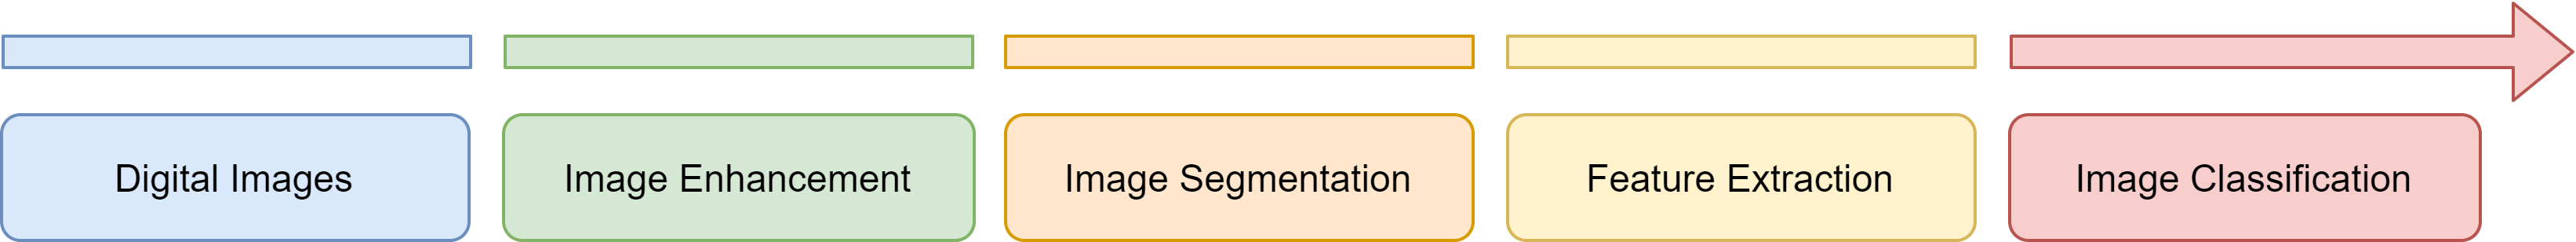
\includegraphics[width=\columnwidth]{images/fig027}
\caption{A simple diagram~\cite{s20143903} for the proposed model pipeline of breast cancer detection. First of all, digital images are acquired. Second, image enhancement must be proceeded. Third, computing image segmentation. Fourth, extraction of features. Fifth and final, classification of images.}
\label{fig:fig027}
\end{figure}
%%%%%%%%%%%%%%%%%%%%%%%%%%%%%%%%%%%%%%%%%%%%%%%%%%%

Several works~\cite{ammar2015semantically, wang2018support, milosevic2017comparison} are addressing many methods for the early detection of breast cancer lesions.
The following sections address each work that is already implemented, or will be implemented, in the work developed under this thesis.
A model for the classification problem was already combined with an intelligent agent and was evaluated (Chapter~\ref{chap:chap005} and Chapter~\ref{chap:chap006}) by clinicians according to early developments of the thesis.
However, the integration of a segmentation model into an intelligent agent is still in progress.
In this work, a classifier was first integrated (Chapter~\ref{chap:chap005}) as a result of clinicians' priority for information concerning the \ac{BI-RADS} classification.
Thus, the segmentation problem is not yet integrated here and will be further addressed (Chapter~\ref{chap:chap008}) as future work.

Although several works~\cite{sharma2020model, 9247957} are arguing to follow a specific pipeline (Figure~\ref{fig:fig027}), it is not mandatory for staying strict to that order, like other authors did~\cite{8451510, AGRAWAL201927}.
During the development and integration of these methods, the order of each process can be changed without loosing model accuracy~\cite{8462671}.
In fact, this thesis is focused on the introduction of intelligent agents as an \ac{HCI} perspective, instead on optimizing the model accuracy.
Therefore, jumping to the final stage of the pipeline (Figure~\ref{fig:fig027}), and start from the end, will be fair to cover the thesis main concerns.

Regarding the above pipeline order ({\it i.e.}, segmentation, feature extraction and classification), each process can be fulfilled separately~\cite{8451510, AGRAWAL201927} and brought together~\cite{10.1007/978-3-030-00934-2_99} in the end of the thesis.
For a proper patient diagnostic, the final classification is actually the most important task~\cite{BHARDWAJ20154611}.
Specifically, the use case achieved from an automatic classification (\ac{BI-RADS}) is the process in which clinicians~\cite{goldenberg2011computer} are informed of the final diagnostic results.
That said, a use case for patient's classification is of a chief importance for the clinicians' workflow~\cite{10.1117/12.2081576}.

In this thesis, the segmentation will support the process of making an intelligent agent more explainable (\ac{XAI}) and interpretable~\cite{8622433}.
For instance, the segmentation can inform the clinician where the lesions are and why ({\it e.g.}, with colours and heatmaps) is the \ac{BI-RADS} so high.
However, segmentation models are more challenging to train~\cite{hesamian2019deep}.
Due to a lack of the available data~\cite{ahmed2020images}, segmentation models are hard to accurately implement in comparison to classification models for the medical imaging domain~\cite{murtaza2019deep}.
One important fact is that image-level labels (weak annotations)~\cite{10.1145/3373017.3373051}, cumming from the classification process, are easier to get for the training set~\cite{TAJBAKHSH2020101693}.
To train a model, the segmentation process is more time-consuming and manual lesion annotations are harder to get from clinicians~\cite{10.1007/978-3-030-59719-1_44}.
Hence, the work under this thesis started first by developing intelligent agents to inform clinicians about the patient classification.

\subsection{Segmentation}
\label{sec:sec003007001}

The above section described several literature works and challenges that this thesis must address to integrate classification and segmentation models into intelligent agents for a proper medical imaging diagnosis.
In this section, the document focus on the works~\cite{7412749, Dabbous397} that will promote and motivate the future integration of segmentation models.
Specifically, one motivation to that integration will be to provide clinicians the visualization of lesions, making these models infer their decisions~\cite{CHOUGRAD201819, doi:10.1148/radiol.2018181371}.
Additionally, the use of these detected lesions can be further applied to aid the training of \acp{DNN}~\cite{8032490, 8861376}.
In this thesis, a multimodality HyperDenseNet~\cite{8515234} model is proposed to be integrated and to solve the segmentation problem.
The task will be to segment inputs of breast images into binary lesion masks, such as masses and microcalcifications.
However, these are just future thoughts being out of the scope of this document, which is describing the work achieved until now.
Therefore, the next section will address important literature for what was done until now under this thesis.

\subsection{Classification}
\label{sec:sec003007002}

From the literature, recent proposed \ac{DenseNet}~\cite{Huang_2017_CVPR} is one of the most used \ac{CNN} structures for the classification of lesions in medical imaging~\cite{LIU2019e271}.
The model connects all the preceding layers as the input for certain layer, which can strengthen feature propagation ({\it e.g.}, {\it radiomics}) and alleviate the gradient vanishing problem~\cite{10.1145/3136755.3143016}.
Furthermore, due to the feature reuse, the \ac{DenseNet} model only needs to learn a small set of new features in each layer.
Thus, the model requires fewer parameters than traditional \acp{CNN}, which is more suitable for small datasets, such as the one created under this thesis.
In this thesis work, a multimodality \ac{DenseNet} model was integrated to solve the classification problem.
The task is to classify inputs of \ac{MG} (both in \ac{CC} and \ac{MLO}), \ac{US}, and \ac{MRI} images.
Along with ground-truth of masses and microcalcifications, the masks of the model can classify (either normal, benign, or malign) into the correct class.

\section{Published Datasets}
\label{sec:sec003008}

In breast screening, published research results are difficult to replicate due to the lack of datasets in the area of \acp{CDSSe}~\cite{lee2017curated}.
Most of the used segmentation (Section~\ref{sec:sec003007001}) and classification (Section~\ref{sec:sec003007002}) methods are evaluated on private datasets~\cite{SADAF2011457} or on unspecified subsets of public databases~\cite{https://doi.org/10.1118/1.4921612}.
These methods are integrated as algorithms for a proper \ac{CADe} and \ac{CADx} on breast cancer and are designed to assist clinicians for a better diagnostic interpretation.
Despite promising results, current \ac{CADe} systems are limited by high \ac{FP} rates~\cite{NISHIKAWA20141320}, and \ac{CADx} systems for breast screening are not yet approved for clinical use because of the lack of available data~\cite{10.1145/3079765}.

Few well-curated public datasets and databases have been provided for breast screening community.
These include INbreast~\cite{MOREIRA2012236}, \ac{MIAS}~\cite{7813261} and \ac{DDSM}~\cite{shen2019deep}.
Although these public datasets are useful, they are limited in terms of data accessibility, completeness and size.
Moreover, datasets are limited in terms of single-modality images ({\it i.e.}, on \ac{MG}-only information) and do not provide any co-variables\footnotemark[10] of the patients.
Such information, is so important to clinicians' workflow.
Furthermore, most researchers are using these datasets without leveraging its images for a variety of reasons~\cite{lee2017curated}.
For instance, the \ac{ROI} annotations for the abnormalities in \ac{DDSM} were provided to indicate a general position of lesions, but not a precise segmentation and classification for them.
Therefore, in this thesis it was also developed a tool (Chapter~\ref{chap:chap004}) that is generating a novel dataset jointly with clinicians.
This feature is covering the implementation problem and limitations of algorithms for accurate feature extraction.

%%%%%%%%%%%%%%%%%%%%%%%%%%%%%%%%%%%%%%%%%%%%%%%%%%%
\footnotetext[10]{The hazard of patient diagnosis must be modelled as a function of several co-variables, such as pathological results, age, morbidity, patient behaviours ({\it e.g.}, smoking), tumour history, between others. Current datasets do not contain any information about these co-variables. A prognostic model that predicts the final diagnostic result and aids in primary clinicians' decision-making must have into consideration these co-variables for early breast cancer detection.}
%%%%%%%%%%%%%%%%%%%%%%%%%%%%%%%%%%%%%%%%%%%%%%%%%%%